% Created by tikzDevice version 0.12.3.1 on 2022-07-27 11:01:32
% !TEX encoding = UTF-8 Unicode
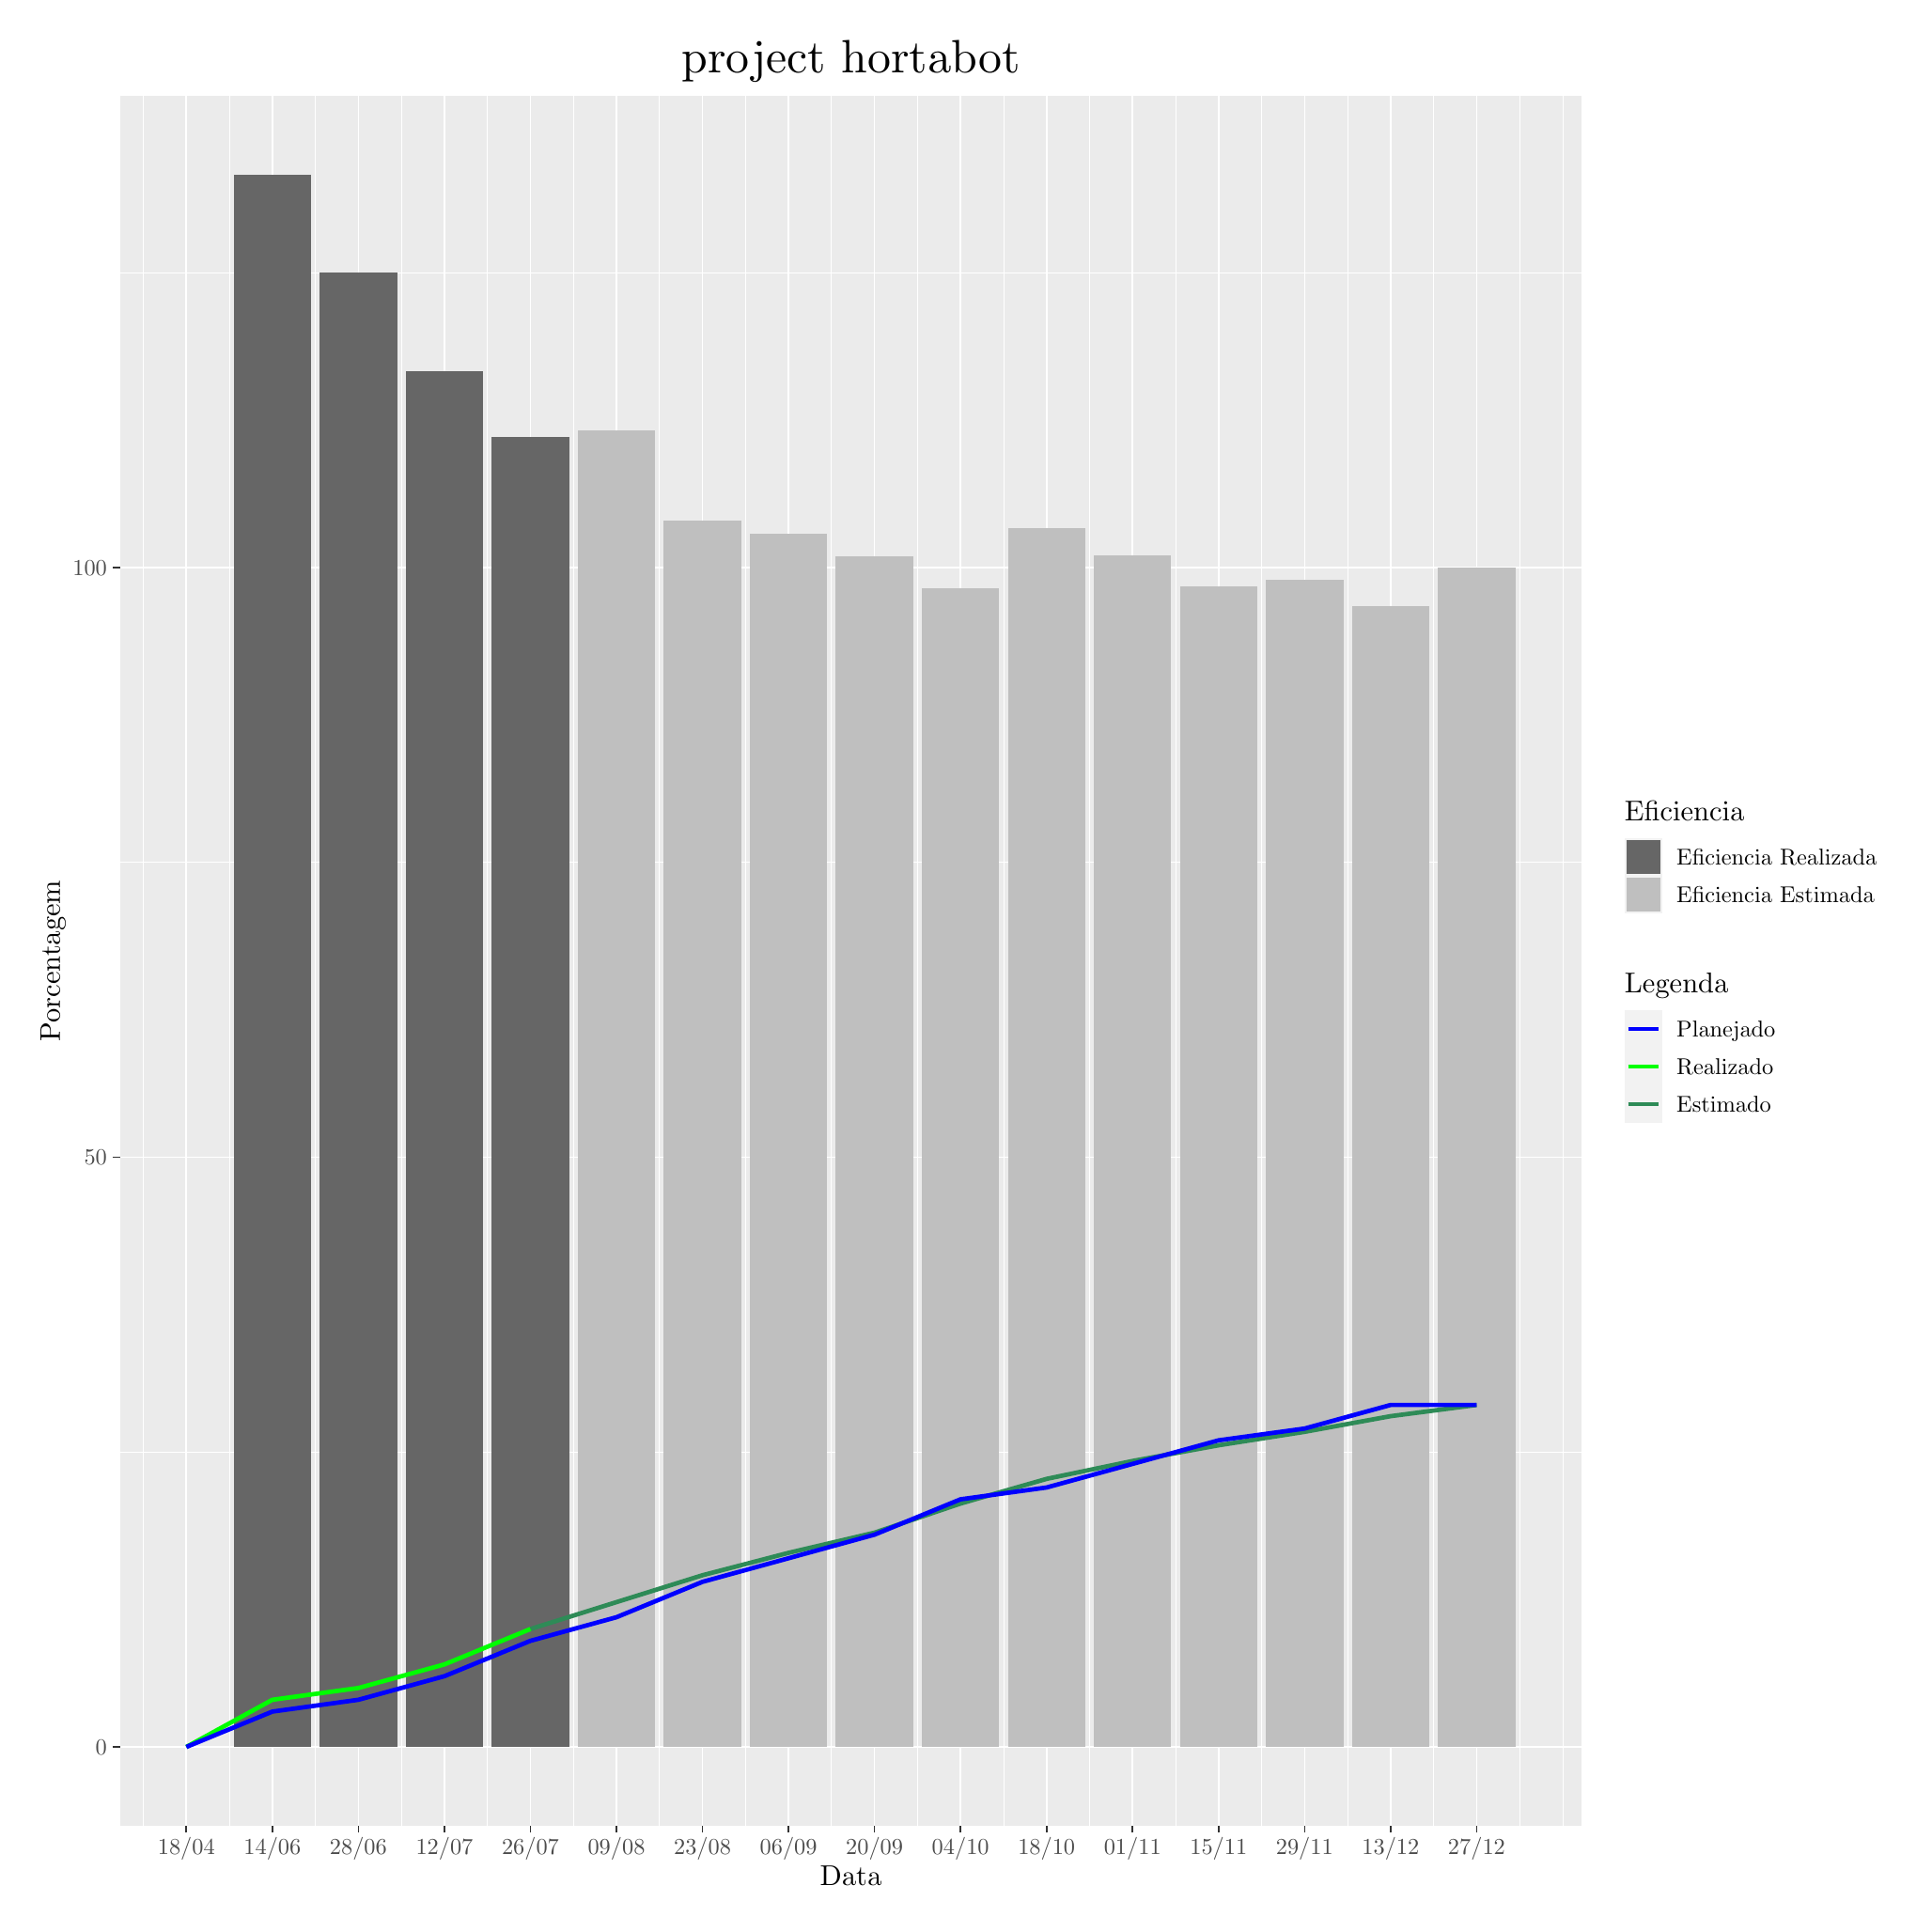
\begin{tikzpicture}[x=1pt,y=1pt]
\definecolor{fillColor}{RGB}{255,255,255}
\path[use as bounding box,fill=fillColor,fill opacity=0.00] (0,0) rectangle (722.70,722.70);
\begin{scope}
\path[clip] (  0.00,  0.00) rectangle (722.70,722.70);
\definecolor{drawColor}{RGB}{255,255,255}
\definecolor{fillColor}{RGB}{255,255,255}

\path[draw=drawColor,line width= 0.6pt,line join=round,line cap=round,fill=fillColor] (  0.00,  0.00) rectangle (722.70,722.70);
\end{scope}
\begin{scope}
\path[clip] ( 36.11, 30.69) rectangle (598.26,695.80);
\definecolor{fillColor}{gray}{0.92}

\path[fill=fillColor] ( 36.11, 30.69) rectangle (598.26,695.80);
\definecolor{drawColor}{RGB}{255,255,255}

\path[draw=drawColor,line width= 0.3pt,line join=round] ( 36.11,174.29) --
	(598.26,174.29);

\path[draw=drawColor,line width= 0.3pt,line join=round] ( 36.11,401.04) --
	(598.26,401.04);

\path[draw=drawColor,line width= 0.3pt,line join=round] ( 36.11,627.78) --
	(598.26,627.78);

\path[draw=drawColor,line width= 0.3pt,line join=round] ( 45.12, 30.69) --
	( 45.12,695.80);

\path[draw=drawColor,line width= 0.3pt,line join=round] ( 78.20, 30.69) --
	( 78.20,695.80);

\path[draw=drawColor,line width= 0.3pt,line join=round] (111.28, 30.69) --
	(111.28,695.80);

\path[draw=drawColor,line width= 0.3pt,line join=round] (144.36, 30.69) --
	(144.36,695.80);

\path[draw=drawColor,line width= 0.3pt,line join=round] (177.44, 30.69) --
	(177.44,695.80);

\path[draw=drawColor,line width= 0.3pt,line join=round] (210.51, 30.69) --
	(210.51,695.80);

\path[draw=drawColor,line width= 0.3pt,line join=round] (243.59, 30.69) --
	(243.59,695.80);

\path[draw=drawColor,line width= 0.3pt,line join=round] (276.67, 30.69) --
	(276.67,695.80);

\path[draw=drawColor,line width= 0.3pt,line join=round] (309.75, 30.69) --
	(309.75,695.80);

\path[draw=drawColor,line width= 0.3pt,line join=round] (342.82, 30.69) --
	(342.82,695.80);

\path[draw=drawColor,line width= 0.3pt,line join=round] (375.90, 30.69) --
	(375.90,695.80);

\path[draw=drawColor,line width= 0.3pt,line join=round] (408.98, 30.69) --
	(408.98,695.80);

\path[draw=drawColor,line width= 0.3pt,line join=round] (442.06, 30.69) --
	(442.06,695.80);

\path[draw=drawColor,line width= 0.3pt,line join=round] (475.13, 30.69) --
	(475.13,695.80);

\path[draw=drawColor,line width= 0.3pt,line join=round] (508.21, 30.69) --
	(508.21,695.80);

\path[draw=drawColor,line width= 0.3pt,line join=round] (541.29, 30.69) --
	(541.29,695.80);

\path[draw=drawColor,line width= 0.3pt,line join=round] (574.37, 30.69) --
	(574.37,695.80);

\path[draw=drawColor,line width= 0.3pt,line join=round] (590.90, 30.69) --
	(590.90,695.80);

\path[draw=drawColor,line width= 0.6pt,line join=round] ( 36.11, 60.92) --
	(598.26, 60.92);

\path[draw=drawColor,line width= 0.6pt,line join=round] ( 36.11,287.66) --
	(598.26,287.66);

\path[draw=drawColor,line width= 0.6pt,line join=round] ( 36.11,514.41) --
	(598.26,514.41);

\path[draw=drawColor,line width= 0.6pt,line join=round] ( 61.66, 30.69) --
	( 61.66,695.80);

\path[draw=drawColor,line width= 0.6pt,line join=round] ( 94.74, 30.69) --
	( 94.74,695.80);

\path[draw=drawColor,line width= 0.6pt,line join=round] (127.82, 30.69) --
	(127.82,695.80);

\path[draw=drawColor,line width= 0.6pt,line join=round] (160.90, 30.69) --
	(160.90,695.80);

\path[draw=drawColor,line width= 0.6pt,line join=round] (193.97, 30.69) --
	(193.97,695.80);

\path[draw=drawColor,line width= 0.6pt,line join=round] (227.05, 30.69) --
	(227.05,695.80);

\path[draw=drawColor,line width= 0.6pt,line join=round] (260.13, 30.69) --
	(260.13,695.80);

\path[draw=drawColor,line width= 0.6pt,line join=round] (293.21, 30.69) --
	(293.21,695.80);

\path[draw=drawColor,line width= 0.6pt,line join=round] (326.28, 30.69) --
	(326.28,695.80);

\path[draw=drawColor,line width= 0.6pt,line join=round] (359.36, 30.69) --
	(359.36,695.80);

\path[draw=drawColor,line width= 0.6pt,line join=round] (392.44, 30.69) --
	(392.44,695.80);

\path[draw=drawColor,line width= 0.6pt,line join=round] (425.52, 30.69) --
	(425.52,695.80);

\path[draw=drawColor,line width= 0.6pt,line join=round] (458.59, 30.69) --
	(458.59,695.80);

\path[draw=drawColor,line width= 0.6pt,line join=round] (491.67, 30.69) --
	(491.67,695.80);

\path[draw=drawColor,line width= 0.6pt,line join=round] (524.75, 30.69) --
	(524.75,695.80);

\path[draw=drawColor,line width= 0.6pt,line join=round] (557.83, 30.69) --
	(557.83,695.80);
\definecolor{fillColor}{gray}{0.40}

\path[fill=fillColor] ( 79.86, 60.92) rectangle (109.63,665.57);

\path[fill=fillColor] (112.93, 60.92) rectangle (142.70,627.78);

\path[fill=fillColor] (146.01, 60.92) rectangle (175.78,589.99);

\path[fill=fillColor] (179.09, 60.92) rectangle (208.86,564.80);
\definecolor{fillColor}{gray}{0.75}

\path[fill=fillColor] (212.17, 60.92) rectangle (241.94,567.18);

\path[fill=fillColor] (245.24, 60.92) rectangle (275.01,532.55);

\path[fill=fillColor] (278.32, 60.92) rectangle (308.09,527.45);

\path[fill=fillColor] (311.40, 60.92) rectangle (341.17,518.69);

\path[fill=fillColor] (344.48, 60.92) rectangle (374.25,506.63);

\path[fill=fillColor] (377.55, 60.92) rectangle (407.32,529.46);

\path[fill=fillColor] (410.63, 60.92) rectangle (440.40,519.13);

\path[fill=fillColor] (443.71, 60.92) rectangle (473.48,507.08);

\path[fill=fillColor] (476.79, 60.92) rectangle (506.56,509.71);

\path[fill=fillColor] (509.86, 60.92) rectangle (539.63,499.55);

\path[fill=fillColor] (542.94, 60.92) rectangle (572.71,514.41);
\definecolor{drawColor}{RGB}{46,139,87}

\path[draw=drawColor,line width= 1.7pt,line join=round] (193.97,106.27) --
	(227.05,116.61) --
	(260.13,126.95) --
	(293.21,135.56) --
	(326.28,143.32) --
	(359.36,154.52) --
	(392.44,164.00) --
	(425.52,170.89) --
	(458.59,176.92) --
	(491.67,182.09) --
	(524.75,188.12) --
	(557.83,192.43);
\definecolor{drawColor}{RGB}{0,255,0}

\path[draw=drawColor,line width= 1.7pt,line join=round] ( 61.66, 60.92) --
	( 94.74, 79.06) --
	(127.82, 83.59) --
	(160.90, 92.66) --
	(193.97,106.27);
\definecolor{drawColor}{RGB}{0,0,255}

\path[draw=drawColor,line width= 1.7pt,line join=round] ( 61.66, 60.92) --
	( 94.74, 74.52) --
	(127.82, 79.06) --
	(160.90, 88.13) --
	(193.97,101.73) --
	(227.05,110.80) --
	(260.13,124.41) --
	(293.21,133.48) --
	(326.28,142.55) --
	(359.36,156.15) --
	(392.44,160.69) --
	(425.52,169.76) --
	(458.59,178.83) --
	(491.67,183.36) --
	(524.75,192.43) --
	(557.83,192.43);
\end{scope}
\begin{scope}
\path[clip] (  0.00,  0.00) rectangle (722.70,722.70);
\definecolor{drawColor}{gray}{0.30}

\node[text=drawColor,anchor=base east,inner sep=0pt, outer sep=0pt, scale=  0.88] at ( 31.16, 57.89) {0};

\node[text=drawColor,anchor=base east,inner sep=0pt, outer sep=0pt, scale=  0.88] at ( 31.16,284.63) {50};

\node[text=drawColor,anchor=base east,inner sep=0pt, outer sep=0pt, scale=  0.88] at ( 31.16,511.38) {100};
\end{scope}
\begin{scope}
\path[clip] (  0.00,  0.00) rectangle (722.70,722.70);
\definecolor{drawColor}{gray}{0.20}

\path[draw=drawColor,line width= 0.6pt,line join=round] ( 33.36, 60.92) --
	( 36.11, 60.92);

\path[draw=drawColor,line width= 0.6pt,line join=round] ( 33.36,287.66) --
	( 36.11,287.66);

\path[draw=drawColor,line width= 0.6pt,line join=round] ( 33.36,514.41) --
	( 36.11,514.41);
\end{scope}
\begin{scope}
\path[clip] (  0.00,  0.00) rectangle (722.70,722.70);
\definecolor{drawColor}{gray}{0.20}

\path[draw=drawColor,line width= 0.6pt,line join=round] ( 61.66, 27.94) --
	( 61.66, 30.69);

\path[draw=drawColor,line width= 0.6pt,line join=round] ( 94.74, 27.94) --
	( 94.74, 30.69);

\path[draw=drawColor,line width= 0.6pt,line join=round] (127.82, 27.94) --
	(127.82, 30.69);

\path[draw=drawColor,line width= 0.6pt,line join=round] (160.90, 27.94) --
	(160.90, 30.69);

\path[draw=drawColor,line width= 0.6pt,line join=round] (193.97, 27.94) --
	(193.97, 30.69);

\path[draw=drawColor,line width= 0.6pt,line join=round] (227.05, 27.94) --
	(227.05, 30.69);

\path[draw=drawColor,line width= 0.6pt,line join=round] (260.13, 27.94) --
	(260.13, 30.69);

\path[draw=drawColor,line width= 0.6pt,line join=round] (293.21, 27.94) --
	(293.21, 30.69);

\path[draw=drawColor,line width= 0.6pt,line join=round] (326.28, 27.94) --
	(326.28, 30.69);

\path[draw=drawColor,line width= 0.6pt,line join=round] (359.36, 27.94) --
	(359.36, 30.69);

\path[draw=drawColor,line width= 0.6pt,line join=round] (392.44, 27.94) --
	(392.44, 30.69);

\path[draw=drawColor,line width= 0.6pt,line join=round] (425.52, 27.94) --
	(425.52, 30.69);

\path[draw=drawColor,line width= 0.6pt,line join=round] (458.59, 27.94) --
	(458.59, 30.69);

\path[draw=drawColor,line width= 0.6pt,line join=round] (491.67, 27.94) --
	(491.67, 30.69);

\path[draw=drawColor,line width= 0.6pt,line join=round] (524.75, 27.94) --
	(524.75, 30.69);

\path[draw=drawColor,line width= 0.6pt,line join=round] (557.83, 27.94) --
	(557.83, 30.69);
\end{scope}
\begin{scope}
\path[clip] (  0.00,  0.00) rectangle (722.70,722.70);
\definecolor{drawColor}{gray}{0.30}

\node[text=drawColor,anchor=base,inner sep=0pt, outer sep=0pt, scale=  0.88] at ( 61.66, 19.68) {18/04};

\node[text=drawColor,anchor=base,inner sep=0pt, outer sep=0pt, scale=  0.88] at ( 94.74, 19.68) {14/06};

\node[text=drawColor,anchor=base,inner sep=0pt, outer sep=0pt, scale=  0.88] at (127.82, 19.68) {28/06};

\node[text=drawColor,anchor=base,inner sep=0pt, outer sep=0pt, scale=  0.88] at (160.90, 19.68) {12/07};

\node[text=drawColor,anchor=base,inner sep=0pt, outer sep=0pt, scale=  0.88] at (193.97, 19.68) {26/07};

\node[text=drawColor,anchor=base,inner sep=0pt, outer sep=0pt, scale=  0.88] at (227.05, 19.68) {09/08};

\node[text=drawColor,anchor=base,inner sep=0pt, outer sep=0pt, scale=  0.88] at (260.13, 19.68) {23/08};

\node[text=drawColor,anchor=base,inner sep=0pt, outer sep=0pt, scale=  0.88] at (293.21, 19.68) {06/09};

\node[text=drawColor,anchor=base,inner sep=0pt, outer sep=0pt, scale=  0.88] at (326.28, 19.68) {20/09};

\node[text=drawColor,anchor=base,inner sep=0pt, outer sep=0pt, scale=  0.88] at (359.36, 19.68) {04/10};

\node[text=drawColor,anchor=base,inner sep=0pt, outer sep=0pt, scale=  0.88] at (392.44, 19.68) {18/10};

\node[text=drawColor,anchor=base,inner sep=0pt, outer sep=0pt, scale=  0.88] at (425.52, 19.68) {01/11};

\node[text=drawColor,anchor=base,inner sep=0pt, outer sep=0pt, scale=  0.88] at (458.59, 19.68) {15/11};

\node[text=drawColor,anchor=base,inner sep=0pt, outer sep=0pt, scale=  0.88] at (491.67, 19.68) {29/11};

\node[text=drawColor,anchor=base,inner sep=0pt, outer sep=0pt, scale=  0.88] at (524.75, 19.68) {13/12};

\node[text=drawColor,anchor=base,inner sep=0pt, outer sep=0pt, scale=  0.88] at (557.83, 19.68) {27/12};
\end{scope}
\begin{scope}
\path[clip] (  0.00,  0.00) rectangle (722.70,722.70);
\definecolor{drawColor}{RGB}{0,0,0}

\node[text=drawColor,anchor=base,inner sep=0pt, outer sep=0pt, scale=  1.10] at (317.19,  7.64) {Data};
\end{scope}
\begin{scope}
\path[clip] (  0.00,  0.00) rectangle (722.70,722.70);
\definecolor{drawColor}{RGB}{0,0,0}

\node[text=drawColor,rotate= 90.00,anchor=base,inner sep=0pt, outer sep=0pt, scale=  1.10] at ( 13.08,363.24) {Porcentagem};
\end{scope}
\begin{scope}
\path[clip] (  0.00,  0.00) rectangle (722.70,722.70);
\definecolor{fillColor}{RGB}{255,255,255}

\path[fill=fillColor] (609.26,375.97) rectangle (717.20,431.09);
\end{scope}
\begin{scope}
\path[clip] (  0.00,  0.00) rectangle (722.70,722.70);
\definecolor{drawColor}{RGB}{0,0,0}

\node[text=drawColor,anchor=base west,inner sep=0pt, outer sep=0pt, scale=  1.10] at (614.76,416.95) {Eficiencia};
\end{scope}
\begin{scope}
\path[clip] (  0.00,  0.00) rectangle (722.70,722.70);
\definecolor{fillColor}{gray}{0.95}

\path[fill=fillColor] (614.76,395.93) rectangle (629.22,410.38);
\end{scope}
\begin{scope}
\path[clip] (  0.00,  0.00) rectangle (722.70,722.70);
\definecolor{fillColor}{gray}{0.40}

\path[fill=fillColor] (615.48,396.64) rectangle (628.51,409.67);
\end{scope}
\begin{scope}
\path[clip] (  0.00,  0.00) rectangle (722.70,722.70);
\definecolor{fillColor}{gray}{0.40}

\path[fill=fillColor] (615.48,396.64) rectangle (628.51,409.67);
\end{scope}
\begin{scope}
\path[clip] (  0.00,  0.00) rectangle (722.70,722.70);
\definecolor{fillColor}{gray}{0.95}

\path[fill=fillColor] (614.76,381.47) rectangle (629.22,395.93);
\end{scope}
\begin{scope}
\path[clip] (  0.00,  0.00) rectangle (722.70,722.70);
\definecolor{fillColor}{gray}{0.75}

\path[fill=fillColor] (615.48,382.18) rectangle (628.51,395.21);
\end{scope}
\begin{scope}
\path[clip] (  0.00,  0.00) rectangle (722.70,722.70);
\definecolor{fillColor}{gray}{0.75}

\path[fill=fillColor] (615.48,382.18) rectangle (628.51,395.21);
\end{scope}
\begin{scope}
\path[clip] (  0.00,  0.00) rectangle (722.70,722.70);
\definecolor{drawColor}{RGB}{0,0,0}

\node[text=drawColor,anchor=base west,inner sep=0pt, outer sep=0pt, scale=  0.88] at (634.72,400.12) {Eficiencia Realizada};
\end{scope}
\begin{scope}
\path[clip] (  0.00,  0.00) rectangle (722.70,722.70);
\definecolor{drawColor}{RGB}{0,0,0}

\node[text=drawColor,anchor=base west,inner sep=0pt, outer sep=0pt, scale=  0.88] at (634.72,385.67) {Eficiencia Estimada};
\end{scope}
\begin{scope}
\path[clip] (  0.00,  0.00) rectangle (722.70,722.70);
\definecolor{fillColor}{RGB}{255,255,255}

\path[fill=fillColor] (609.26,295.40) rectangle (678.22,364.97);
\end{scope}
\begin{scope}
\path[clip] (  0.00,  0.00) rectangle (722.70,722.70);
\definecolor{drawColor}{RGB}{0,0,0}

\node[text=drawColor,anchor=base west,inner sep=0pt, outer sep=0pt, scale=  1.10] at (614.76,350.83) {Legenda};
\end{scope}
\begin{scope}
\path[clip] (  0.00,  0.00) rectangle (722.70,722.70);
\definecolor{fillColor}{gray}{0.95}

\path[fill=fillColor] (614.76,329.80) rectangle (629.22,344.26);
\end{scope}
\begin{scope}
\path[clip] (  0.00,  0.00) rectangle (722.70,722.70);
\definecolor{drawColor}{RGB}{0,0,255}

\path[draw=drawColor,line width= 1.7pt,line join=round] (616.21,337.03) -- (627.77,337.03);
\end{scope}
\begin{scope}
\path[clip] (  0.00,  0.00) rectangle (722.70,722.70);
\definecolor{drawColor}{RGB}{0,0,255}

\path[draw=drawColor,line width= 1.7pt,line join=round] (616.21,337.03) -- (627.77,337.03);
\end{scope}
\begin{scope}
\path[clip] (  0.00,  0.00) rectangle (722.70,722.70);
\definecolor{drawColor}{RGB}{0,0,255}

\path[draw=drawColor,line width= 1.7pt,line join=round] (616.21,337.03) -- (627.77,337.03);
\end{scope}
\begin{scope}
\path[clip] (  0.00,  0.00) rectangle (722.70,722.70);
\definecolor{fillColor}{gray}{0.95}

\path[fill=fillColor] (614.76,315.35) rectangle (629.22,329.80);
\end{scope}
\begin{scope}
\path[clip] (  0.00,  0.00) rectangle (722.70,722.70);
\definecolor{drawColor}{RGB}{0,255,0}

\path[draw=drawColor,line width= 1.7pt,line join=round] (616.21,322.58) -- (627.77,322.58);
\end{scope}
\begin{scope}
\path[clip] (  0.00,  0.00) rectangle (722.70,722.70);
\definecolor{drawColor}{RGB}{0,255,0}

\path[draw=drawColor,line width= 1.7pt,line join=round] (616.21,322.58) -- (627.77,322.58);
\end{scope}
\begin{scope}
\path[clip] (  0.00,  0.00) rectangle (722.70,722.70);
\definecolor{drawColor}{RGB}{0,255,0}

\path[draw=drawColor,line width= 1.7pt,line join=round] (616.21,322.58) -- (627.77,322.58);
\end{scope}
\begin{scope}
\path[clip] (  0.00,  0.00) rectangle (722.70,722.70);
\definecolor{fillColor}{gray}{0.95}

\path[fill=fillColor] (614.76,300.90) rectangle (629.22,315.35);
\end{scope}
\begin{scope}
\path[clip] (  0.00,  0.00) rectangle (722.70,722.70);
\definecolor{drawColor}{RGB}{46,139,87}

\path[draw=drawColor,line width= 1.7pt,line join=round] (616.21,308.12) -- (627.77,308.12);
\end{scope}
\begin{scope}
\path[clip] (  0.00,  0.00) rectangle (722.70,722.70);
\definecolor{drawColor}{RGB}{46,139,87}

\path[draw=drawColor,line width= 1.7pt,line join=round] (616.21,308.12) -- (627.77,308.12);
\end{scope}
\begin{scope}
\path[clip] (  0.00,  0.00) rectangle (722.70,722.70);
\definecolor{drawColor}{RGB}{46,139,87}

\path[draw=drawColor,line width= 1.7pt,line join=round] (616.21,308.12) -- (627.77,308.12);
\end{scope}
\begin{scope}
\path[clip] (  0.00,  0.00) rectangle (722.70,722.70);
\definecolor{drawColor}{RGB}{0,0,0}

\node[text=drawColor,anchor=base west,inner sep=0pt, outer sep=0pt, scale=  0.88] at (634.72,334.00) {Planejado};
\end{scope}
\begin{scope}
\path[clip] (  0.00,  0.00) rectangle (722.70,722.70);
\definecolor{drawColor}{RGB}{0,0,0}

\node[text=drawColor,anchor=base west,inner sep=0pt, outer sep=0pt, scale=  0.88] at (634.72,319.55) {Realizado};
\end{scope}
\begin{scope}
\path[clip] (  0.00,  0.00) rectangle (722.70,722.70);
\definecolor{drawColor}{RGB}{0,0,0}

\node[text=drawColor,anchor=base west,inner sep=0pt, outer sep=0pt, scale=  0.88] at (634.72,305.09) {Estimado};
\end{scope}
\begin{scope}
\path[clip] (  0.00,  0.00) rectangle (722.70,722.70);
\definecolor{drawColor}{RGB}{0,0,0}

\node[text=drawColor,anchor=base,inner sep=0pt, outer sep=0pt, scale=  1.80] at (317.19,704.80) {project hortabot};
\end{scope}
\end{tikzpicture}
